\section{Input stage med pre-amp og DC-offset}
Systemet skal kunne modtage et signal fra en lydkilde, som afspiller lyd i det menneskeligt hørbare område. 
Før signalet kan videreføres til anti aliasing filtrene, skal der være en mulighed for eventuelt at forstærke signalet med en operationsforstærker. 
På den måde kan en fuld opløsning opnås ved den senere AD konvertering. 
\newline
Et almindeligt analogt lydsignal har generelt frekvenser mellem 20Hz og 20kHz, som svarer til det menneskeligt hørbare område. 
Signalets spænding varierer for forskellige kilder. 
Der findes ingen officiel standard, men en del forbruger-elektronik har typisk en maksimal amplitude på 0,447V.\cite{wikiLine} 
\newline
Til forstærkningen benyttes en aktiv operationsforstærker med 3,3V single-supply. 
Men indgangssignalet fra lydkilden vil svinge omkring 0V. 
Derfor skal signalet have et offset, da signalet ellers vil blive klippet hver gang det går under 0V, da operationsforstærkeren ved single-supply ikke har mulighed for at have negative udgangssignaler. 
Det ønskes at indgangssignalet har mulighed for at svinge både så højt og lavt som muligt, så offsettet designes til at være symmetrisk, med respekt til  forsyningsspændingen. 
\begin{equation}
	{V_{offset}} = \frac{V_{supply}}{2} = \frac{3,3\text{V}}{2} = 1,65\text{V}
\end{equation}
Ved et offset på 1,65V kan signalet ideelt have en maksimal amplitude på 1,65V. 
%Herfra skal den valgte operationsforstærkers output swing i forhold til dens forsyningsspænding trækkes fra. (vender tilbage til det her når op-amp skal vælges)
Ved at opbygge en spændingsdeler, kan offsettet skabes. Kredsløbet ses på figur \ref{fig:modtagerKreds}.

\subsubsection{Valg af operationsforstærker til forstærkning af indgangssignalet}
Operationsforstærkeren som skal forstærke signalet vælges ud fra en række krav. 

\begin{itemize}
	\item Forstærkeren skal kunne forsynes med  single-supply 3,3V
	\item Båndbredden skal være minimum 44,1 kHz.
	\item Rail to rail voltage swing skal være så stort som muligt. 
	\item Slew rate skal være hurtig nok til at signalet ikke forvrænges. 
	\item Komponenten skal være tilgængelig som SMD komponent. 
\end{itemize}
Den nødvendige slew rate kan beregnes ved formel \ref{eq:slewrate}.\cite{slewrate}
\begin{equation}
\label{eq:slewrate}
\text{Slew rate} = 2 \pi \cdot f_{maks} \cdot V_{maks} = 2\pi \cdot 44,1\text{kHz} \cdot 1,65\text{V} = 0,46\text{V/\micro S}
\end{equation}
\husk{JES}{Er det egentligt kun 20kHz her?}
Ud fra kravene vælges operationsforstærkeren AD8031 som SMD komponent. 
Forstærkeren kan operere ved en single-supply forsyning ned til 2,7V, har 80MHz -3dB båndbredde ved en forstærkning på 1 og en slew rate på 30V/\micro S. 
Forstærkerens output swing ligger inden for 20mV af rail-spændingen. Ved 3,3V ligger spændingsvidden således fra 0,02V til 3,28V. 
Forstærkerens specifikationer overgår kravene med en stor margen. 
Det var ikke muligt at finde en anden operationsforstærker som var tilgængelig som SMD, der både havde en acceptabel slew rate, samt muligheden for en single-supply forsyningsspænding på 3,3V. 
Havde der været mere tid, kunne det have været bestilt hjem. 

\subsubsection{Beregning af forstærkning}
For at forstærke signalet, opsættes operationsforstærkeren som en ikke-inverterende forstærker. 
Da indgangssignalets maksimale amplitude vil variere alt efter input, skal forstærkningens styrke kunne justeres. 
Derfor sættes en variabel modstand i serie med feedback-modstanden. 
Det ses på figur \ref{fig:modtagerKreds}. 
Den variable modstand kan gå fra at være tæt på kortsluttet og op til 100k$\Omega$.
For at undgå en kortslutning fra operationsforstærkerens output og til den inverterende indgang, er den variable modstand sat i serie med en feedback-modstand på 5k$\Omega$. 
$R_2$ er valgt til 47k$\Omega$, så modstanden matcher modstanden fra højpasfilteret. 
I formel \ref{eq:Aminfors} og \ref{eq:Aminfors} ses den mulige maksimum- og minimumsforstærkning.

\begin{equation}
\label{eq:Aminfors}
A_{maks.} = 1 + \frac{R_{feedback} + R_{variabel}}{R_2} = 1 + \frac{5\text{k} \Omega + 100\text{k} \Omega}{47\text{k} \Omega} = 3,23
\end{equation}
\begin{equation}
\label{Amaksfors}
A_{min.} = 1 + \frac{R_{feedback}}{R_2} = 1 + \frac{5\text{k} \Omega}{47\text{k} \Omega} = 1,11
\end{equation}

\subsubsection{Højpas filter-design}
Mellem inputtet og operationsforstærkeren sidder en kapacitor, som blokerer for al DC fra indgangssignalet. 
Som det ses på figur \ref{fig:modtagerKreds}, vil kapacitoren og modstandene fra offsettet udgøre et højpas filter. 
Filterets knækfrekvens sættes så lavt, at alle frekvenser i det hørbare område ikke påvirkes. 
Ved AC-analyse kortsluttet forsyningen. Derfor sidder modstandene $R1$ og $R2$ parallelt.
Det endelige kredsløb er kopieret, således der er to udgange for at opnå stereo. 
\begin{equation}
f_c = \frac{1}{2\pi R C} = \frac{1}{2 \pi \frac{1}{\frac{1}{47k \Omega}+\frac{1}{47k \Omega}}  470\text{nF}} = 14,1\text{Hz}
\end{equation}

\begin{figure}[h]
\caption{Kredsløbet for modtageren af indgangssignalet.}
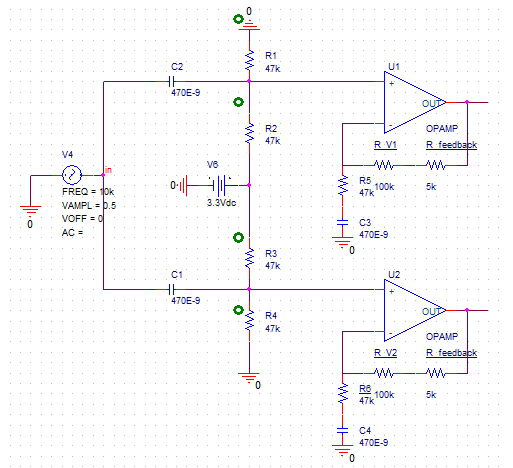
\includegraphics[width=0.8\linewidth]{./billeder/Modtager.png}
\label{fig:modtagerKreds}
\end{figure}

\husk{Jes}{Hvis der er problemer med antal sider, kan der henvises til et bilag med det samlede print i stedet. Opdatering: Bilag med samlet print er ved at blive lavet. }

\section{Output stage}